\section{Foundation's of Cloud and Fog Computing}

%-----------------------------------------------------------------subsection1

\subsection{Challenges of Cloud Computing: Why Fog Computing?}
Cloud computing has several challenges like communication cost, downtime, high latency, processing of big data, security and privacy, and traffic congestion.
Most of the IoT applications require low latency. But, the cloud cannot guarantee it because of the huge geographical distance between the Data Centers (DCs) (e.g., Amazon web services (AWS) and Google cloud) and the End-User (EU).
Technical hitches and interruptions might occur in any internet-based system for no reason leading to downtime. 
The private data of a single user is transferred through globally connected channels along with the vast data of other users. The system might prone to cyber-attacks and even data loss.  
Besides, total greenhouse gas emissions caused by DCs i.e., the carbon footprint is additionally a significant challenge, as DCs are operated day-and-night.
The huge geographical distance between DCs and the EU results in high latency and Quality-of-Service (QoS) degradation, which are not appropriate for time-sensitive service requests \cite{mukherjee2018survey}, \cite{nat}. \par

To overcome this, fog computing was introduced as an alternative approach to support geographically distributed, latency-sensitive, and QoS-aware IoT applications.
Fog is an extension of cloud computing. The term 'fog computing' was introduced by Cisco, explaining that all the functionalities of cloud computing are extended to the edge of the network. 
Fog nodes are geographically much closer to the EU than DCs providing better computation, storage facilities, and networking services. Fog computing is a highly virtualized platform that resides between the EU and DCs \cite{mukherjee2018survey}, \cite{nat}. 

%-----------------------------------------------------------------subsection2

\subsection{Fog Computing}

%------------------------------subsubsection2.1

\subsubsection{Definition}

According to \cite{openfog2017openfog} 'Fog computing' is "A horizontal, system-level architecture that distributes computing, storage, control and networking functions closer to the users along a cloud-to-thing continuum."

%------------------------------subsubsection2.2

\subsubsection{Pillars of OpenFog}

Fog computing is for IoT, 5G, and Artificial Intelligence (AI) systems that need SCALE \cite{ambrose}. SCALE is the OpenFog term for Security, Cognition, Agility, Latency, and Efficiency \cite{mukherjee2018survey}.

\begin{figure}[H]
    \centering
    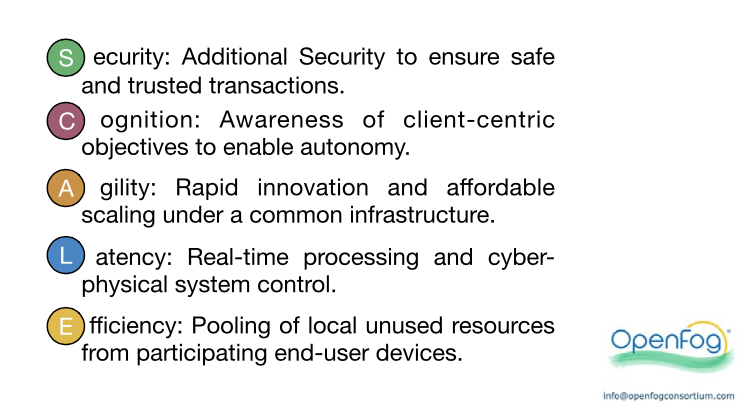
\includegraphics[width=.6\linewidth]{image/SCALE.png}
    \caption{SCALE}
    \caption*{img src: \cite{mukherjee2018survey}}
    \label{fig:scale}
\end{figure}

Fig. \ref{fig:pillars of openfog} shows the eight pillars of OpenFog. Fog nodes have several capabilities like storage, computation, networking, hardware, and software segments \cite{youtube}. \par

Security plays an important role in making systems trustworthy. And it is achieved with attestation, privacy, cryptographic techniques, and so on.
Scalability is incredibly important, especially within the IoT, where there might be billions of things to connect to IoT networks and also the fog.
And scalability makes sure that the system can control, configure, manage, orchestrate all of the capabilities and provides scalable performance. Openness is additionally important \cite{youtube}. 

\begin{figure}[H]
    \centering
    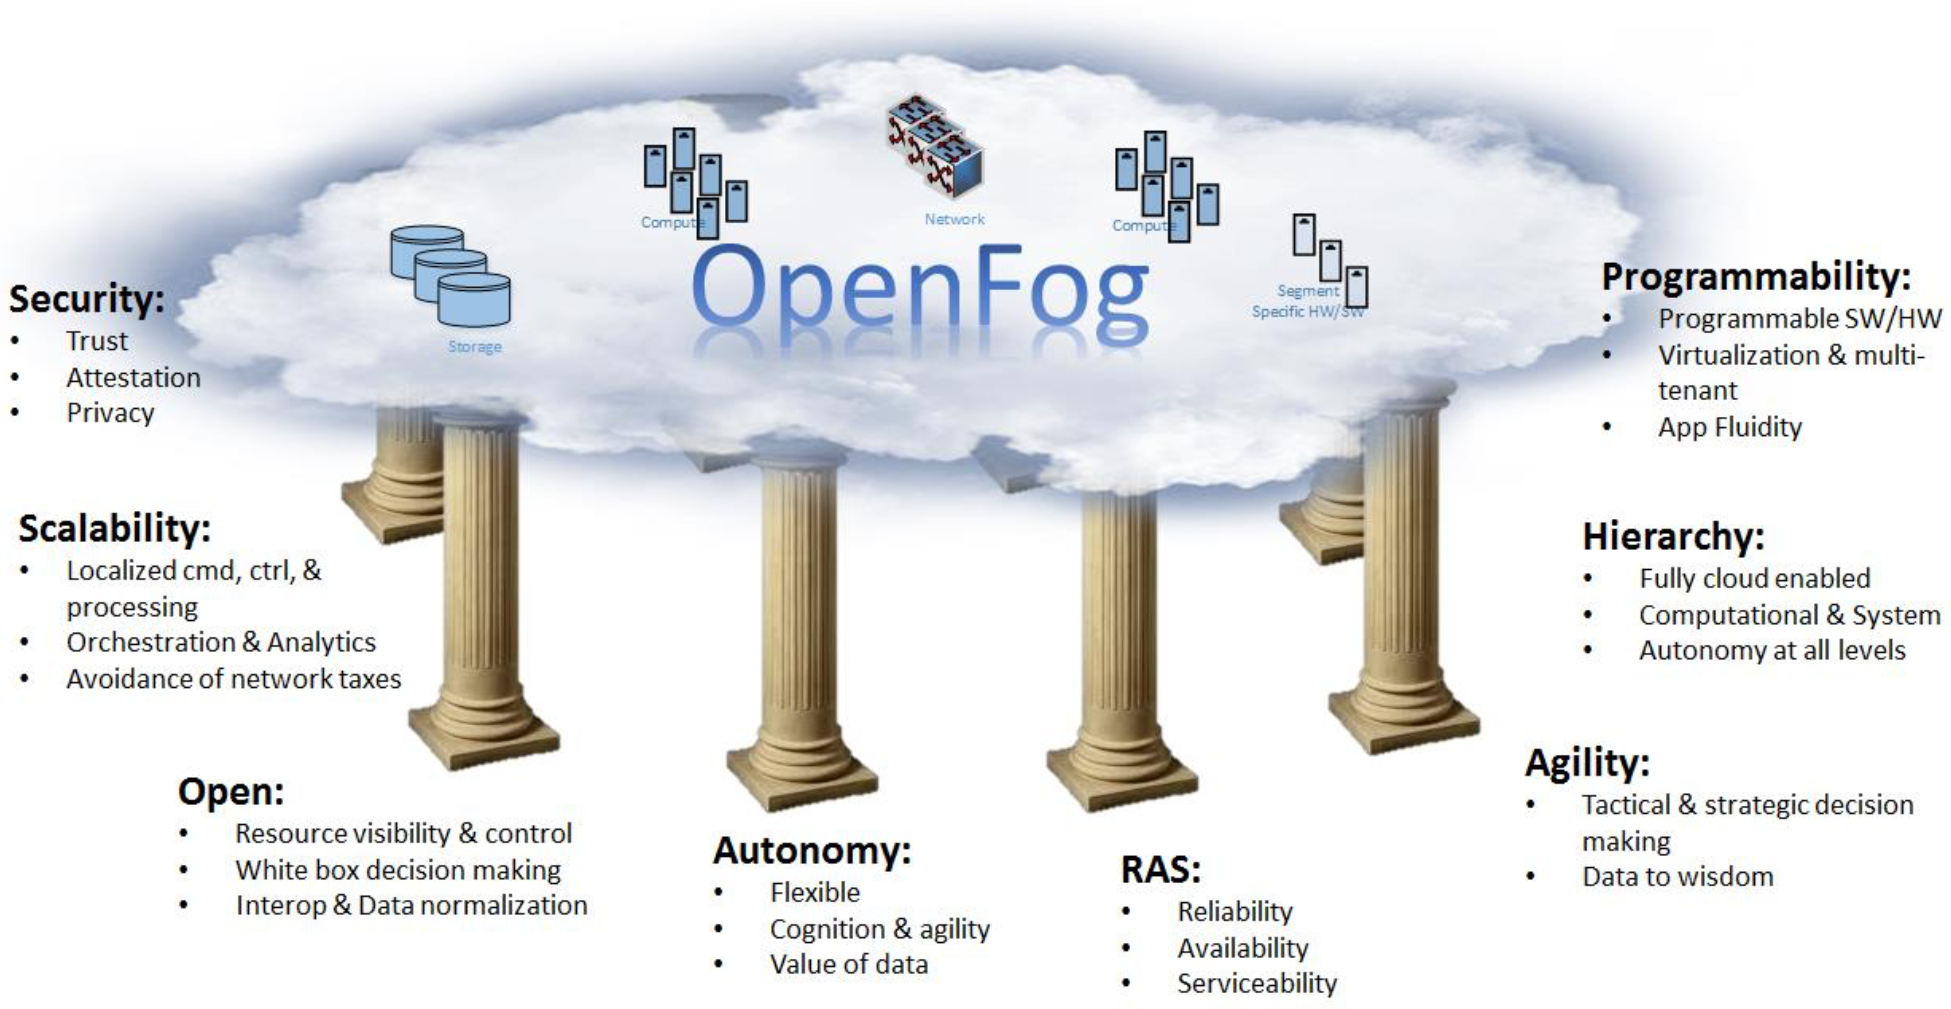
\includegraphics[width=\textwidth]{image/Pillars of OpenFog.png}
    \caption{Pillars of OpenFog}
    \caption*{img src: \cite{openfog2016openfog}}
    \label{fig:pillars of openfog}
\end{figure}

Fog nodes have to be autonomous, which means a fog network needs to be flexible and should be able to manage its cognitive abilities. 
RAS is a term for reliability, availability, and serviceability. It explains what fog does to keep itself reliable and trustworthy. 
Agility explains that a fog network should be able to make decisions tactically and strategically, which helps in converting data to wisdom or knowledge. 
Hierarchy explains that fog is fully cloud-enabled and distributes computational and system capabilities and also autonomous at all levels. 
Fog is a fully programmable architecture that provides programmable software and hardware capabilities, supports virtualization, multi-tenant operation, and app fluidity \cite{youtube}.

%------------------------------subsubsection2.3

\subsubsection{Main features of fog computing}

Fig. \ref{fig:scale} shows some of the advantages of fog computing like security, cognition, agility, latency, and efficiency \cite{openfog2016openfog}.

The main features of fog computing are \cite{mukherjee2018survey}, \cite{nat}, \cite{far}:
\begin{itemize}
    \item capacity of processing a high number of nodes,
    \item connection loss is impossible,
    \item end-device mobility,
    \item heterogeneity,
    \item low latency and location awareness,
    \item no bandwidth issues,
    \item privacy control,
    \item real-time applications,
    \item reduced operation costs,
    \item supports geographic distribution, and
    \item wireless access               
\end{itemize}

Fog computing is capable of processing a high number of nodes \cite{mukherjee2018survey}. Connection loss is impossible because of multiple interconnected channels \cite{nat}. Fog computing provides end-device mobility. Fog network connects heterogeneous devices irrespective of hardware and operating system \cite{madakam2018fog}. Fog computing can guarantee low latency and location awareness, as fog nodes are physically closer to the EU \cite{nat}, \cite{10.1145/3022636.3022649}. No bandwidth issues as data is fragmented and then combined while delivering \cite{nat}. Privacy control can be achieved by analyzing data locally instead of sending it to the cloud \cite{far}. Has endless capabilities to process real-time applications \cite{mukherjee2018survey}. Processing of preferred data locally, instead of sending it to the cloud, can save network bandwidth and also reduces operating costs \cite{far}. Fog computing supports geographic distribution and wireless access \cite{mukherjee2018survey}. 

%------------------------------subsubsection2.4

\subsubsection{Differences between cloud computing and fog computing}

The differences between cloud computing and fog computing \cite{mukherjee2018survey}, \cite{nat}, \cite{edu} are listed in Table \ref{tab:tab1} below.

\begin{center}
\begin{longtable}{|l|l|l|}
\caption{Comparison of cloud computing and fog computing} \label{tab:tab1} \\

\hline \multicolumn{1}{|c|}{\textbf{Features}} & \multicolumn{1}{c|}{\textbf{Cloud Computing}} & \multicolumn{1}{c|}{\textbf{Fog Computing}} \\ \hline 
\endfirsthead

\multicolumn{3}{c}%
{{\bfseries \tablename\ \thetable{} -- continued from previous page}} \\
\hline \multicolumn{1}{|c|}{\textbf{Features}} & \multicolumn{1}{c|}{\textbf{Cloud Computing}} & \multicolumn{1}{c|}{\textbf{Fog Computing}} \\ \hline  
\endhead

\hline \multicolumn{3}{|r|}{{Continued on next page}} \\ \hline
\endfoot

\hline \hline
\endlastfoot

%Access speed & Depends on VM & High\\
%Applications & Cyber-domain applications & Both Cyber-domain and cyber-physical applications, mainly time-critical applications\\
%Architecture & Centralized & Distributed\\
%Computing manner & Centralized & Both distributed and centralized\\
%Cost of deployment & High & Low\\
%Latency & High & Very low\\
%Maintenance & By technical experts & No human interference\\
%Mobility management & Easy & Hard\\
%Operation & By large companies & By both large and small companies depending on the size\\
%Reliability & High & Low\\
%Resource optimization & Global & Local\\
%Security & Low & Very high\\
%Size of DCs & Very large & Smaller\\

Access speed & Depends on VM & High\\
Architecture & Centralized & Distributed\\
Computing manner & Centralized & Both distributed and centralized\\
Cost of deployment & High & Low\\
Latency & High & Very low\\
Maintenance & By technical experts & No human interference\\
Mobility management & Easy & Hard\\
Reliability & High & Low\\
Resource optimization & Global & Local\\
Security & Low & Very high\\
Size & Very large & Smaller\\

\end{longtable}
\end{center}

Cloud computing supports cyber-domain applications. Whereas, fog computing supports both cyber-domain and cyber-physical applications, mainly time-critical applications.  Cloud is operated by large companies and fog is operated by both large and small companies depending on the size. Even though fog computing provides low latency, cloud computing is more reliable than fog computing. The size of cloud DCs is very large and the size of the fog system is smaller. But, multiple smaller fog nodes form a large fog system \cite{mukherjee2018survey}.

%------------------------------subsubsection2.5

\subsubsection{Fog architecture}

Fog architecture consists of a number of different layers. The most commonly used architectures in fog computing are three-tier architecture and layered architecture. The architectures are discussed in Sec. \ref{sec:3}

%-----------------------------------------------------------------subsection3

\subsection{Cloud Computing}

%------------------------------subsubsection3.1

\subsubsection{Definition}

According to \cite{mell2011nist} "Cloud computing is a model for enabling ubiquitous, convenient, on-demand network access to a shared pool of configurable computing resources (e.g., networks, servers, storage, applications, and services) that can be rapidly provisioned and released with minimal management effort or service provider interaction. This cloud model is composed of five essential characteristics, three service models, and four deployment models.

\begin{itemize}
    \item Essential characteristics: On-demand self-service, broad network access, resource pooling, rapid elasticity, measured service.
    \item Service models: Software as a Service (SaaS), Platform as a Service (PaaS), Infrastructure as a Service (IaaS).
    \item Deployment models: Private cloud, community cloud, public cloud, hybrid cloud."
\end{itemize}

%------------------------------subsubsection3.2

\subsubsection{Service-oriented distributed computing in the cloud}

The objectives are computing, storage, networking, and management on demand (U. Krieger: KTR-Mobicom-M-E). \par
Scalable distributed computing using characteristics like resource pooling. Unlimited storage capacity. The connection between applications and servers is by IP networks (U. Krieger: KTR-Mobicom-M-E). 

%------------------------------subsubsection3.3

\subsubsection{Virtualization}

Types of virtualization in cloud computing are application, network, desktop, and storage virtualization \cite{nam}. \par
The basic virtualization technologies are Virtual Machine (VM) and Docker. \par
A VM also known as a hypervisor is a software or hardware that creates and runs virtual machines \cite{hypervisor}.
A VM imitates the actions of the computer. It runs in the dedicated window and leaves the user with the experience of using the host system. It runs in its own sandbox. Many VMs can run at the same time on the host system. Each VM has it's own OS and shares the hardware of the host system for VM support. The abstraction of hardware reduces costs and  power demand \cite{mic}. 

"Docker allows you to package an application with all of its dependencies into a standardized unit for software development" (Dr. Andreas Schönberger, Großmann, Dr. Kolb, Manner DSG-SOA-M 2020 – 9 – Docker). "Docker containers wrap up a piece of software in a complete filesystem that contains everything it needs to run: code, runtime, system tools, system libraries - anything you can install on a server. This guarantees that it will always run the same, regardless of the environment it is running in" (Dr. Andreas Schönberger, Großmann, Dr. Kolb, Manner DSG-SOA-M 2020 – 9 – Docker). Docker works on build, ship, and run everywhere paradigm (Dr. Andreas Schönberger, Großmann, Dr. Kolb, Manner DSG-SOA-M 2020 – 9 – Docker). The process of deploying applications with the help of containers is called containerization. Containers are flexible, lightweight, loosely coupled, portable, scalable, and secure \cite{doc}. \par

\begin{figure}[H]
    \centering
    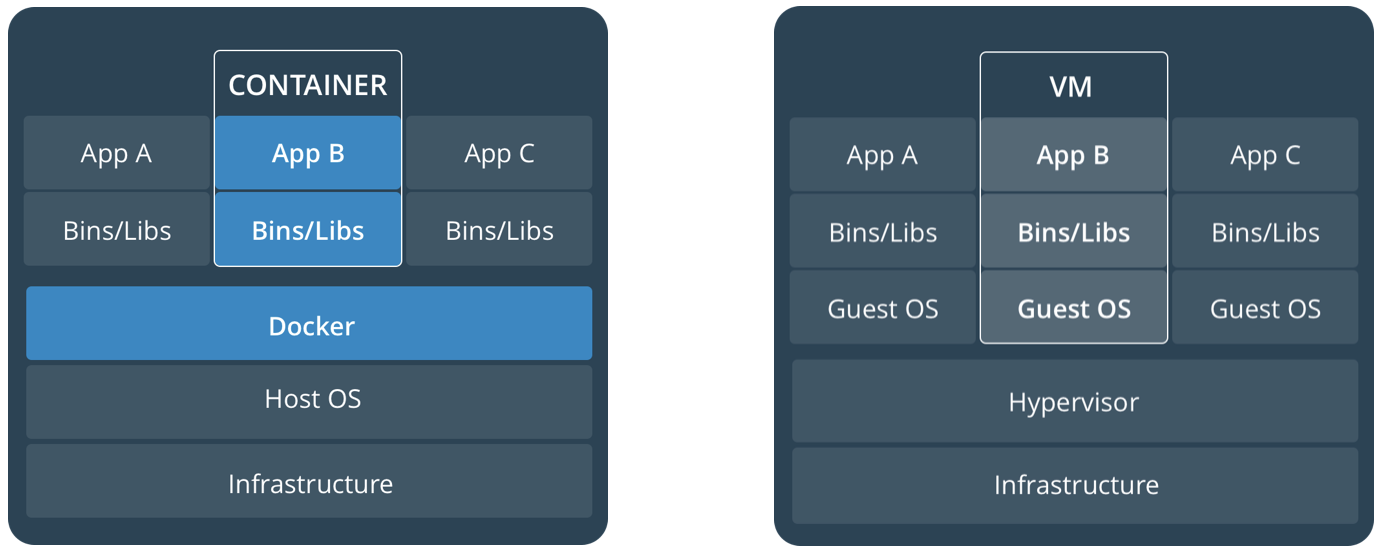
\includegraphics[width=\textwidth]{image/Containers and virtual machines.png}
    \caption{Containers and virtual machines}
    \caption*{img src: \cite{doc}}
    \label{fig:containers and virtual machines}
\end{figure}

Docker containers are lightweight and easy to manage as they share the host OS for isolation support. Besides, VMs are heavy as each VM has its own guest OS. Docker containers are preferred when users have to deploy multiple applications over a single host OS. On the other hand, VMs are preferred when the users have to run applications on different OSs \cite{doc}, \cite{avi}. 

%-----------------------------------------------------------------subsection4

\subsection{Virtualized Fog DCs}

According to \cite{wiki:xxx} "Data center is a pool of resources (computational, storage, network) interconnected using a communication network. Data Center Network (DCN) holds a pivot role in a data center, as it interconnects all of the data center resources together." A DCN is defined by its network topology, protocols, and routing/switching equipment \cite{mukherjee2018survey}. Types of DCN are Three-tier DCN, Fat tree DCN, and Dcell \cite{wiki:xxx}. \par
Fig. \ref{fig:data center virtualization} shows data center virtualization where multiple Virtual Networks (VNs) can be created and implemented independently. VNs can be processed in isolation as they are independent of each other. All the resources are virtualized  in a virtual data center with the help of a hypervisor which makes application deployment easier \cite{mukherjee2018survey}. \par

Server virtualized technologies like VMware and Xen can support the requirements of traditional data centers like high server utilization, performance isolation, and low operation costs. But, they cannot support application deployment, flexibility, and security related issues. So, the main goal of data center virtualization is to address flexibility and efficiency to meet the requirements of Data Service Subscribers (DSSs). Based on the requirements of DSSs, Massive Data Center Operators create (MDCO) a virtualized server \cite{mukherjee2018survey}. 

\begin{figure}[H]
    \centering
    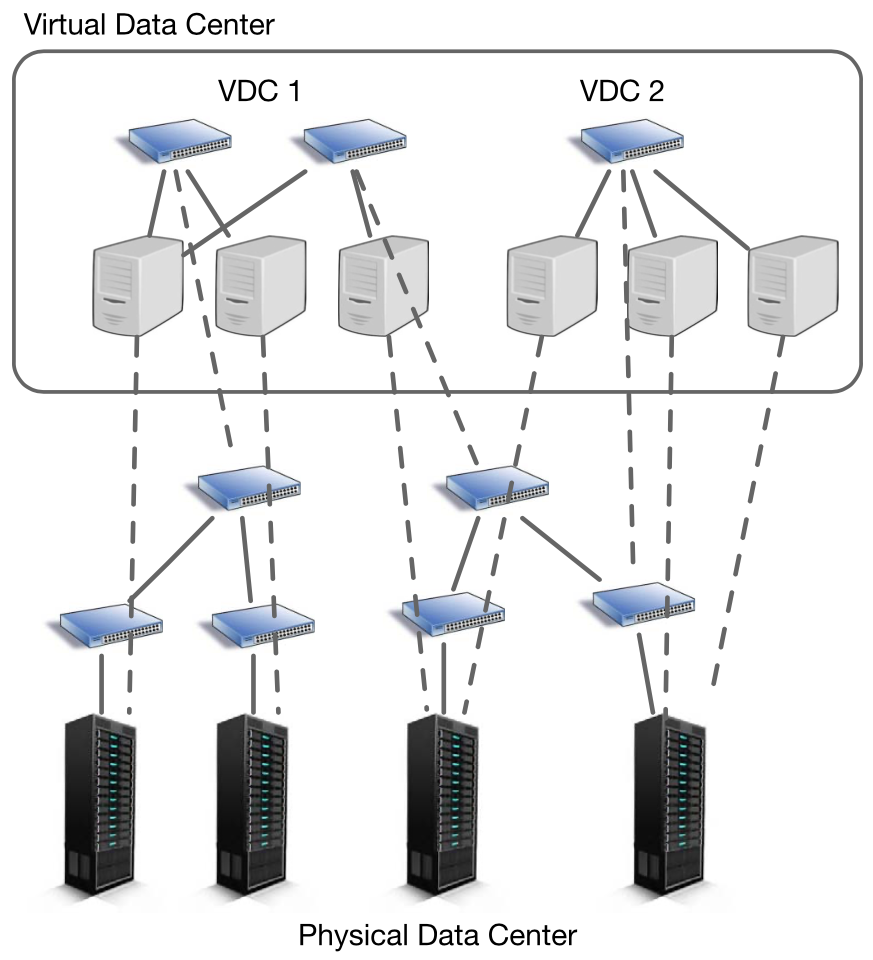
\includegraphics[width=.5\linewidth]{image/Data center virtualization.png}
    \caption{Data center virtualization}
    \caption*{img src: \cite{mukherjee2018survey}}
    \label{fig:data center virtualization}
\end{figure}

One server alone can process the requirements of DSSs, which improves capacity utilization and energy efficiency. Even though a single server can process requirements of multiple DSSs, as massive data centers and DSSs are far from each other, massive data centers may encounter high latency and operation costs. As a solution, fog computing supports multiple virtualized edge data centers to offload the service from massive data centers \cite{mukherjee2018survey}. \par

Fig. \ref{fig:data center networks with fog computing} shows the three-tier architecture where the bottom tier consists of DSSs, the middle tier consists of MDCOs, and the top tier consists of FNs. FNs and MDCOs share computation and storage facilities. And, MDCOs provide latency-sensitive services to the DSSs \cite{mukherjee2018survey}.

\begin{figure}[H]
    \centering
    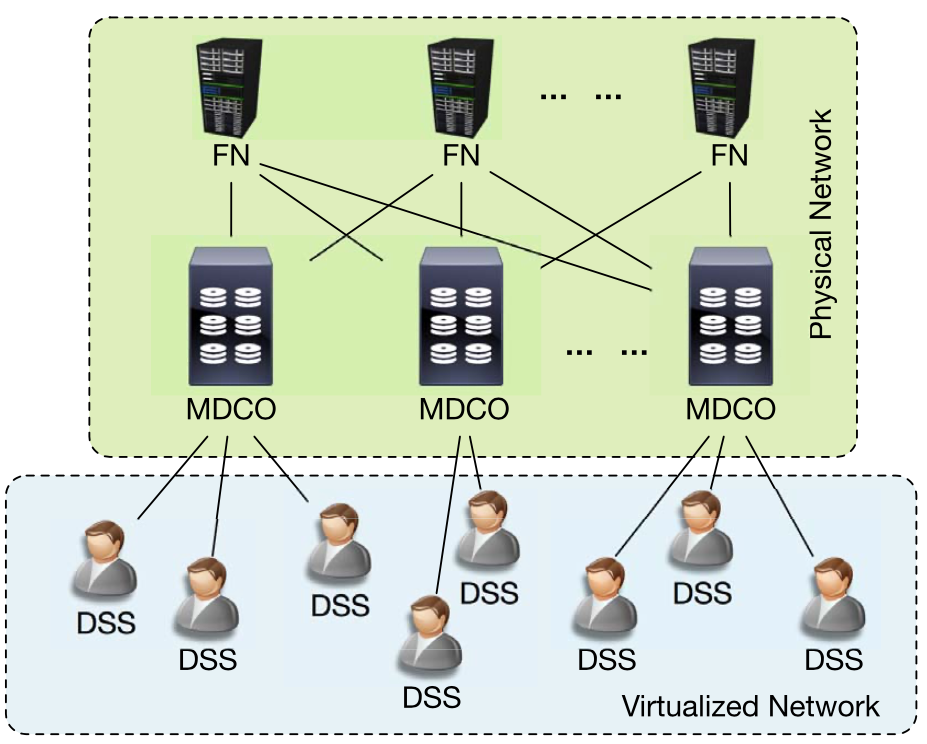
\includegraphics[width=.5\linewidth]{image/Data center networks with fog computing.png}
    \caption{Data center networks with fog computing}
    \caption*{img src: \cite{mukherjee2018survey}}
    \label{fig:data center networks with fog computing}
\end{figure}